\ifsvnmulti
 \svnkwsave{$RepoFile: siminos/lyapunov/QR.tex $}
 \svnidlong
 {$HeadURL$}
 {$LastChangedDate$}
 {$LastChangedRevision$} {$LastChangedBy$}
 \svnid{$Id$}
\fi

\renewcommand{\ssp}{x}            % state space point


\section{Stability in a co-moving frame}
\label{sect:stabComoving}
% Predrag                           		2011-03-05
% moved to here halcrow/blog/TEX/QR.tex		2008-12-07

{\bf Predrag 2011-03-05}
{These appendices contain material that will eventually be returned back to
    ChaosBook.org. Please keep ChaosBook formatting throughout this chapter.
    Thanks!}

%%%%%%%%%%%%%%%%%%%%%%%%%%%%%%%%%%%%%%%%%%%%%%%%%%%%%%%%%%%%%%%%%%%%%%%%%%
\exercise{Stability in a co-moving frame.}{ \label{exer:stabComoving}
% Predrag                           19feb2008
\index{stability|co-moving frame}
\index{|co-moving frame|stability}
    %
\PC{ChaosBook: add this to Problems/exerAppApplic}
%
The {\em \stabmat}(velocity gradient matrix):
\index{matrix!stability}
\index{stability!matrix}
\index{velocity gradient matrix}
% % http://mathworld.wolfram.com/StabilityMatrix.html
% calls this `stability matrix'.
%   }
\beq
{\Mvar}_{ij}(\ssp) = \frac{\pde \vel_i(\ssp)}{\pde \ssp_j  }
\ee{appl:DerMatrix}
The linearized neighborhood is transported by the
{\jacobianM}
% This Jacobian matrix has inherited the name
% {\em fundamental solution matrix} or simply
% {\em fundamental matrix}
% from the theory of linear ODEs.
\index{fundamental matrix}
\beq
\jMps^t_{ij}(\xInit)
  =  \left. {\pde \ssp_i(t) \over \pde \ssp_j} \right|_{\ssp=\xInit}
\, .
\label{appl:hOdes}
\eeq
$\ExpaEig_k$ denotes
the $k$th
{\em eigen\-value}
(multiplier)
 of the finite time
 {\jacobianM} $\jMps^t$,
\index{stability!eigenvalue}
while $\eigExp[k]$ denotes
the $k$th {\em characteristic exponent}
or
{\em characteristic value},
% sometimes the same thing as the {\em Lyapunov exponent}),
with real part $\eigRe[k]$
% is sometimes the same thing as the {\em Lyapunov exponent}),
and phase $\eigIm[k]$:
\index{characteristic!exponent}
\index{characteristic!value}
% \index{Lyapunov exponent}
\beq
\ExpaEig_k
 =
e^{t \eigExp[k]}
 =
e^{t\eigRe[k] +i t\eigIm[k]}
\,.
\ee{appl:stabExpon}
$\derf{t}{\xInit}$ depends on the initial point $\xInit$
and the elapsed time $t$. For notational brevity we tend to
omit this dependence. Projection operator
\beq
{\PP}_i = \prod_{j\not= i}
   \frac{\jMps-\ExpaEig_j \matId }
        {\ExpaEig_i - \ExpaEig_j} \, ,
\ee{appl:stab:3.42}
projects arbitrary $\ssp \in \pS$ onto the $i$th eigenspace
of $\jMps$.

If you are evolving a high-dimensional flow with a handful of
expanding eigen-directions and contracting eigen-directions of
comparable magnitude, and the remaining many contracting eigen-directions
so contracting to be irrelevant. One would like to find a way to
economically evolve a local low-dimensional eigenvector frame of
$\jMps^t$ that keeps track only of these directions.

Initiate this construction by evaluating the leading
eigenvectors for a full-space $\jMps^T$ computed after the flow has
evolved for some typical turnover time $T$, and constructing
projection operators on this subspace by keeping in
\refeq{appl:stab:3.42} only $|\ExpaEig_i| > \ExpaEig_{min}$.

Now find {\em implementable} equations for $\ExpaEig_i$,
${\PP}_i$ time $t$ later.
Assume all relevant eigenvalues are distinct, and
the marginal (symmetry induced) eigenvalues have been eliminated.
If the projection operator notation
${\PP}_i$ is not to your taste, replace it
by left/right eigenvectors $\jEigvecT{i}$, $\jEigvec{j}$.

\begin{itemize}
\item[(a)]
    Show that the $j$th multiplier evolves in the co-moving frame as
\beq
\dot{\ExpaEig}_j = \Mvar_{jj} \ExpaEig_j
    \,,\quad
\Mvar_{jk}= {\PP}_j \Mvar {\PP}_k
    \,,\qquad \mbox{no sum on } j
\,.
\ee{appl:dotLambda}
\item[(b)]
    Show that the $j$th projection operator
    (or eigenvector) evolves as a set of ODEs
\beq
{\PP}_j \dot{\PP}_j  {\PP}_k = %\sum_{k \neq j}
            \frac{\ExpaEig_j}
                 {\ExpaEig_j - \ExpaEig_k} \Mvar_{jk}
    \,,\qquad k \neq j \mbox{, no sum on } j
\,.
\ee{appl:dotP}
\end{itemize}
These coupled ODEs are beguiling but useless for
hyperbolic flows, as $\ExpaEig_j$ contract/expand exponentially
with time, and projection operators become quickly uncomputable due to
numerical under/over flows. One needs to track instead the
finite time Lyapunov exponents
$
\eigExp[k](t) = (1/t) \ln \ExpaEig_k
$
which remain bounded for flows of bounded hyperbolicity.

\begin{itemize}
\item[(c)]
    Show that this is correct (or not):
\beq
\dot{\eigExp}^{(j)} = (\Mvar_{jj} - {\eigExp}^{(j)})/t
\,.
\ee{appl:dotlambda}
Explain the initial conditions.
Is there some smarter way of writing this (redefining time, whatever?)
\item[(d)]
    Write corresponding equations for ${\PP}_j$
    It is not clear that there is
    a sensible way - try keeping\rf{CV93,CBook:appendApplic}
    eigenvectors normalized
     $|\jEigvec{j}| = 1$?
\item[(e)]
    Deal with the complex eigenvalues case?
\item[(f)]
    Discuss likelihood that eigenvalues cross. What
happens to the eigenvectors?
\item[(g)]
    Test your formulation on Lorenz or R\"ossler.
\item[(h)]
    propose alternative, better co-moving frame methods?
\end{itemize}

\hfill Jean-Luc Thiffeault and Predrag Cvitanovi\'c
        }% end \exercise{Stability in a co-moving frame

\solution{exer:stabComoving}{Stability in a co-moving frame.}{
\index{stability|co-moving frame}
\index{|co-moving frame|stability}

See Dieci \etal\rf{DJRV07} on QR method (the paper is on
\HREF{http://www.math.ku.edu/~evanvleck/papers.html}
     {http://www.math.ku.edu/~evanvleck/papers.html})

The issue of projection operators becoming uncomputable due to
numerical under/over flows has been addressed
by Vattay and Cvitanovi\'c\rf{CV93,CBook:appendApplic}.

Recheck - is \refref{Thiffeault2001} or \refref{ThiBoo99} more relevant
here?

    } %end \exercise{Stability in a co-moving frame


\Remarks

\remark{Blah und Bluh.}{ \label{dscr:r:symmCycles}
We conclude with a few comments about
Lagrangian velocity gradient tensor turbulence averaging methods\rf{GLEM07}.
} %end \remark{Cycles and symmetries.}{


\section{Flow linearized about a hyperbolic equilibrium}


\begin{figure}
 % source in /dasbuch/book/FigSrc/inkscape/eqbHypbLin.svg
 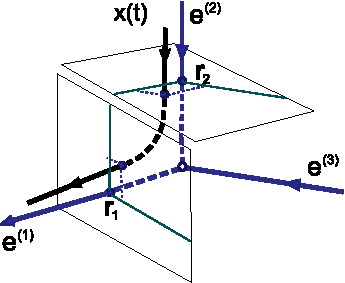
\includegraphics[width=0.45\textwidth]{eqbHypbLin}
  \caption{Linearization of a flow near to an equilibrium:
  the flow is reduced to an analytic map between two
  near Poincar\'e sections, mapping the in-flow into out-flow.
  }\label{f:eqbHypbLin}
\end{figure}
